\section{Graphical user intefrace}
\label{sec:200:gui}

The following section describes the usage of the IBM ExaBounds graphical user interface.

\subsection{Loading application profiles}

IBM ExaBounds can load application profiles in the JSON format generated by IBM Platform-Independent Software Analysis~\cite{Anghel2016} or in the Mathematica format generated by IBM Exascale Extrapolator~\cite{Mariani2016}. This can be used to use ExaBounds to analyze any application that can be analyzed using IBM Platform-Independent Software Analysis. Figure~\ref{fig:200:loadjson} shows the GUI element that can be used to load algorithms. It shows the algorithms already loaded. The \textsc{default} algorithm is loaded by default and contains two profiles of the Graph 500~\cite{Graph500} benchmark set. By clicking \textsc{Import JSON file} a dialog box opens to load new IBM Platform-Independent Software Analysis files in JSON format. Similarly, clicking \textsc{Import mathematica file} allows loading an IBM Exascale Extrapolator file in Mathematica format *.m (by default, IBM Exascale Extrapolator stores data in the \textsc{predictedAlgorithm} symbol).

\begin{figure}
  \centering
  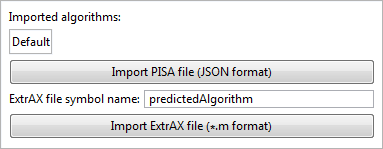
\includegraphics[width=0.6\columnwidth]{img/load-json.png}
  \caption{Import algorithms GUI element.}
  \label{fig:200:loadjson}
\end{figure}

During loading of an input file, several warning messages can be displayed at the bottom of the CDF file. Two types of warning messages can exist: missing properties and invalid data. In case of invalid data, there is a problem with the data in the input file. For example, the summation of all instruction fractions does not add up to 1. % The PISA file or ExtrAX extrapolation models should be inspected and potentially be regenerated.

An example missing properties warning is:
\begin{mma}
	\Warning{AlgorithmFromFileJSON`LoadAlgorithmJSON::missingproperties} The properties \linebreak \{externalLibraryCallCount, instrReuseDistribution, memoryFootprint, mpiCommunicationVector, mpiDataExchanged, mpiInstructionMix, openMPinstructionMix\} were not read correctly for the file: file.out. \\
\end{mma}
The warning states that several properties are missing in the profile file and therefor not loaded. Care should be taken that all properties that are relevant for a specific analysis are loaded for valid performance and power analysis results. Table~\ref{tbl:200:properties} list the common properties\footnote{These properties usually cover several parameters in the profile files.} and for which parts of the models they are used. Note that all properties related to core modeling should always be loaded.

\begin{table}
  \centering
  \small
  \caption{Properties and their use in the analytic models.}
  \label{tbl:200:properties}
  \begin{threeparttable}
    \begin{tabular}{lll}
    	\toprule
      \textbf{Property} & \textbf{Use} & \textbf{Always needed?} \\
      \midrule
      instructionMix & Core modeling & Yes \\
      dataReuseDistribution\tnote{1} & Core modeling & Yes \\
      instrReuseDistribution & Not used & No \\
      memoryFootprint & Not used & No \\
      branchEntropy & Not used & No \\
      bestMisprectionRate & Core modeling & No \\
      ilp & Core modeling & Yes \\
      ilptype & Core modeling & Yes \\
      inorder ilp\tnote{2} & In-order core modeling & No \\
      inorder ilptype\tnote{2} & In-order core modeling & No \\
      registerAccesses & Core modeling & Yes \\
      openMPinstructionMix & Not used & No \\
      mpiInstructionMix & Not used & No \\
      mpiDataExchanged & Not used & No \\
      mpiCommunicationVector & Not used & No \\
      externalLibraryCallCount & Not used & No \\
      processId & Not used & No \\
      threadId & Not used & No \\
      \bottomrule
    \end{tabular}
    \begin{tablenotes}
      \item[1] The data reuse distribution for two cache line sizes (64 and 128) is being read, only one is needed. However, a warning will be generated when only one is available.
      \item[2] Will be deprecated. In-order modeling will be done using the regular ILP parameters.
    \end{tablenotes}
  \end{threeparttable}
\end{table}

\subsection{Loading architectures}

Architectures are also described using JSON files. In total, three different types of JSON files can be loaded: processor architecture files, memory architecture files and network architecture files. Each file contains a set of parameters that describe an architecture, the parameters are described in Appendix~\ref{app:architecture-parameters}. During execution of the models, an processor, memory, and network architecture are combined to describe a complete system.

IBM ExaBounds loads a set of default architectures that can be used. Custom architectures can be loaded using the architecture interface as shown in Figure~\ref{fig:200:loadarchitectures}.

\begin{figure}
  \centering
  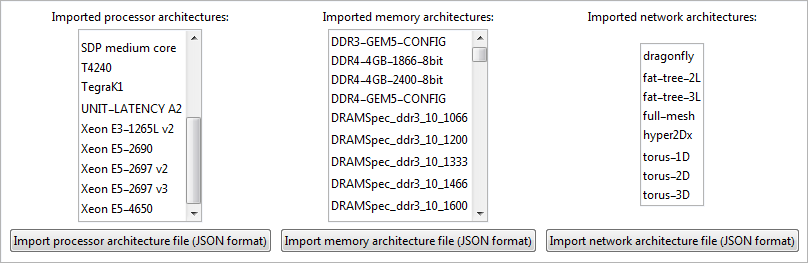
\includegraphics[width=0.95\columnwidth]{img/load-architecture.png}
  \caption{Import architectures GUI element.}
  \label{fig:200:loadarchitectures}
\end{figure}

\subsection{Performing a basic performance and power analysis for a single thread single-node}

\subsubsection{Choosing the architecture}

The first step to do a basic performance and power analysis is to select the architecture to study.
Figure~\ref{fig:200:architecturepicker} shows the architecture selection box. The drop-down menu allows to select any of the predefined machine configurations. By clicking the small downward arrow, a table expands which shows the architectural parameters of the choosen configuration.

\begin{figure}
  \centering
 	\subfloat[Architecture picker]{
		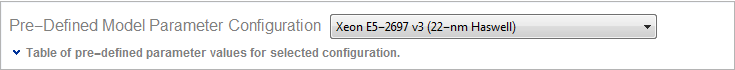
\includegraphics[width=0.98\columnwidth]{img/archpicker.png}
		\label{fig:200:architecturepicker}
	}\\
	\subfloat[Application picker]{
		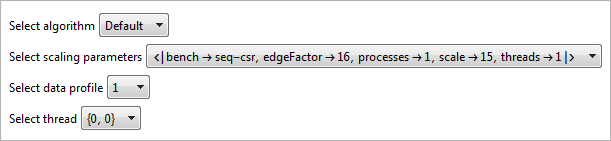
\includegraphics[width=0.8\columnwidth]{img/apppicker.png}
		\label{fig:200:applicationpicker}
	}
	\caption{Selection boxes to select an architecture and algorithm for a basic performance and power analysis.}
	\label{fig:200:architectureapplicationpicker}
\end{figure}

\subsubsection{Choosing the application}

After selection of the architecture, an application can be selected to analyze. Figure~\ref{fig:200:applicationpicker} shows the four selection boxes needed to select a thread from an application. From top to bottom, the four boxes select: the algorithm, an associated set of scaling parameters (e.g., the data size), a data profile (e.g., different runs with different data), and finally a specific thread.

\subsubsection{Results}

After selection, the results update automatically and is presented in two forms: the bottleneck plot and a table.

Figure~\ref{fig:200:bottleneckplot} shows the bottleneck plot of the selected combination of architecture and application. The plot gives insight in the architectural and application parameters that limit the performance of the thread. The blue bullets show absolute constraints, while the orange crosses show relative constraint. The relative constraints are always relative of an absolute constraint: shifting the absolute constraints will also shift the relative constraints. The absolute constraints are independent of each other. In the example, the absolute constraint limiting performance is the ILP per type mem, which indicates that the limited parallelism in the memory access or their long latency is expected to limit performance on a real system. The branch misprediction penalty decreases performance further.

\begin{figure}
  \centering
  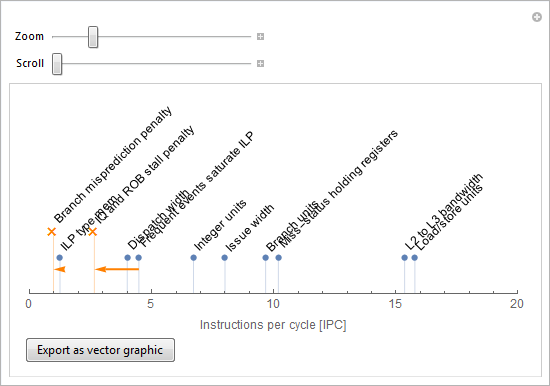
\includegraphics[width=0.7\columnwidth]{img/bottleneckplot.png}
  \caption{Bottleneck plot for the selected architecture and application pair.}
  \label{fig:200:bottleneckplot}
\end{figure}

The results in table-form are shown in Figure~\ref{fig:200:resultstable}. By default, the power analysis using McPAT, and IBM Memory-Scheduler-Agnostic Power Model or CACTI is disabled. By checking the checkbox, the power analysis can be enabled and will run automatically. Please note that this can take some time to finish during which it may appear that the system hangs.

\begin{figure}
  \centering
  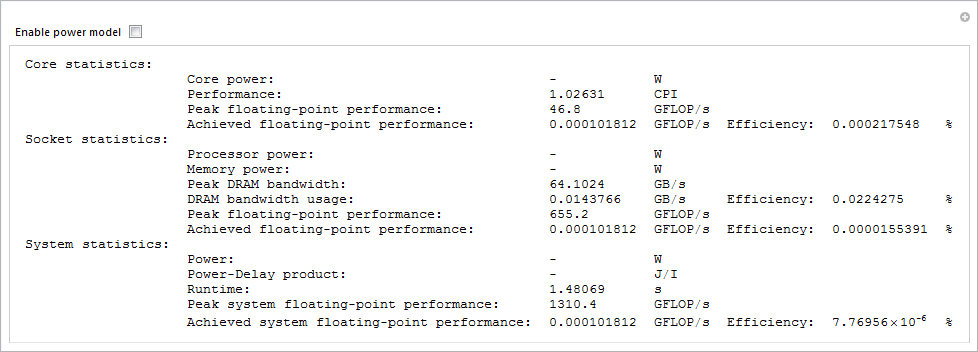
\includegraphics[width=0.9\columnwidth]{img/resultstable.png}
  \caption{Results table for the selected architecture and application pair.}
  \label{fig:200:resultstable}
\end{figure}

\subsection{Multi-core analysis}

A multi-core analysis can be performed using the multi-core GUI interface as is shown in Figure~\ref{fig:200:multicore}. It is a known issue that this interface is sometimes slow to respond.

\begin{figure}
  \centering
  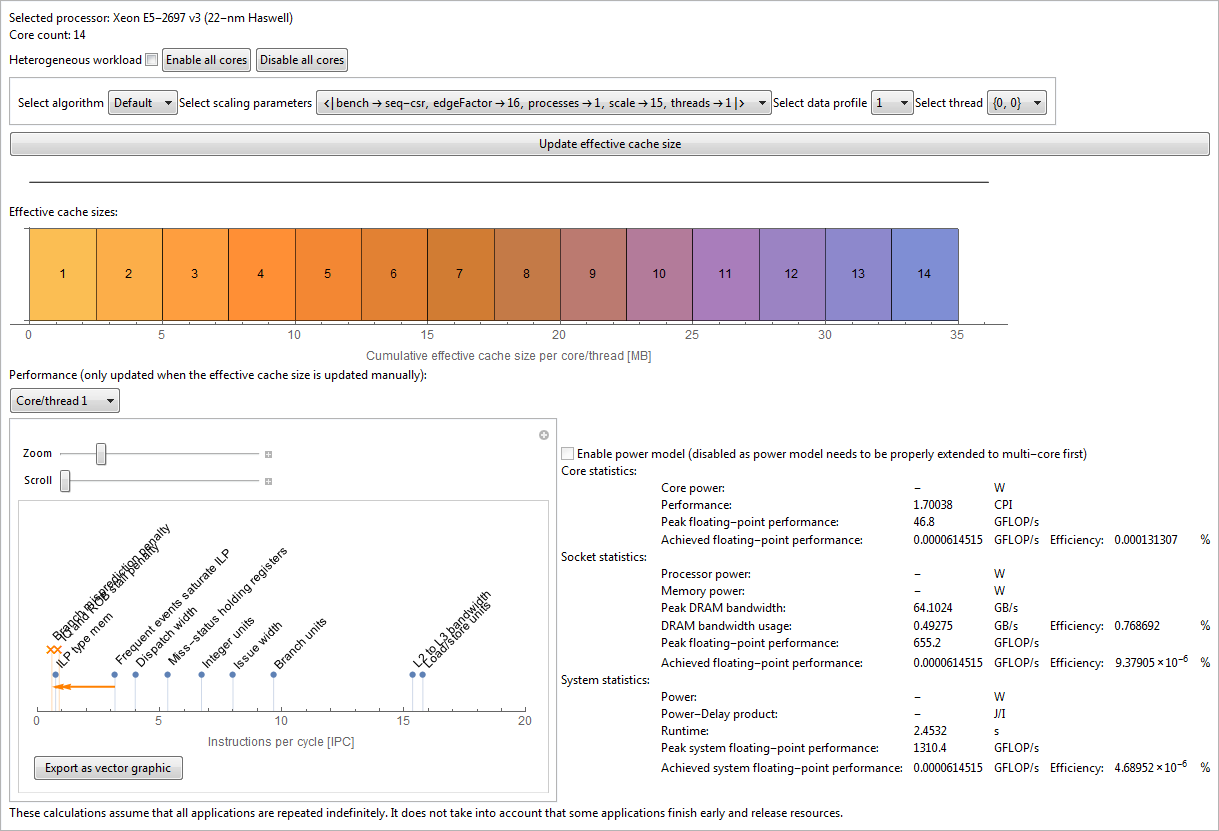
\includegraphics[width=1.0\columnwidth]{img/multicoregui.png}
  \caption{Multi-core analysis GUI and results.}
  \label{fig:200:multicore}
\end{figure}

The first step is to select an architecture with the architecture selection box as shown in Figure~\ref{fig:200:architecturepicker}. Then, the required threads can be selected to run on the target platform. The GUI gives the choice to run a homogeneous workload (all threads the same) or a heterogeneous workload (all threads different). After specifying the right threads, click the ``Update results'' button to recalculate the effective cache size for each thread and update the results. The results will be shown with a similar bottleneck plot and table as shown before.

\subsection{Design-space exploration}

T.b.d.

\subsection{Troubleshooting}

It can happen that external tools like McPAT fail or that for other reasons IBM ExaBounds returns wrong answers due to some error. Usually, re-evaluating the model does not help as IBM ExaBounds caches intermediate results to speed up evaluation. The three buttons at the bottom of the notebook can be used to clear all caches. Notice that this means that all analysis will be performed again.
